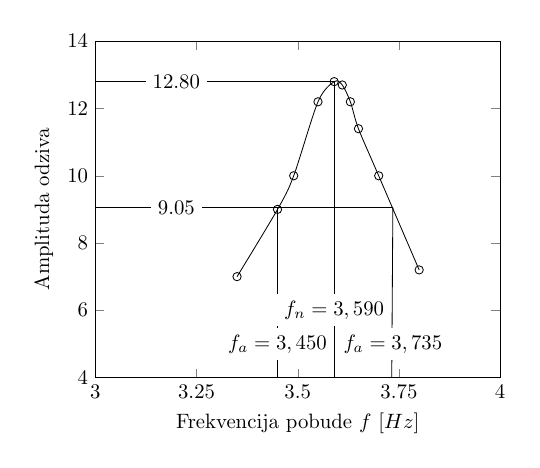
\begin{tikzpicture}[scale=0.75]
    \begin{axis} [
        ylabel = Amplituda odziva,
        xlabel = {Frekvencija pobude $f$ $[Hz]$},
        xmin = 3, xmax = 4,
        ymin = 4, ymax = 14,
        xtick = {3.0, 3.25, 3.5, 3.75, 4.0},
%        grid=both,
     ]
        \draw (3.35, 7)  circle[radius=2pt,fill=none,color=black]; 
        \draw (3.45, 9) circle[radius=2pt,fill=none,color=black];
        \draw (3.49, 10) circle[radius=2pt,fill=none,color=black];
        \draw (3.55,12.2) circle[radius=2pt,fill=none,color=black];
        \draw (3.59,12.8) circle[radius=2pt,fill=none,color=black];
        \draw (3.61,12.7) circle[radius=2pt,fill=none,color=black];
        \draw (3.63,12.2) circle[radius=2pt,fill=none,color=black];
        \draw (3.65,11.4) circle[radius=2pt,fill=none,color=black];
        \draw (3.7,10) circle[radius=2pt,fill=none,color=black];
        \draw (3.8,7.2) circle[radius=2pt,fill=none,color=black];
        
        \draw plot [smooth] coordinates{
            (3.35, 7)
            (3.45, 9) 
            (3.49, 10) 
            (3.55,12.2) 
            (3.59,12.8) 
            (3.61,12.7) 
            (3.63,12.2) 
            (3.65,11.4) 
            (3.7,10) 
            (3.8,7.2) 
        };

        %amplituda rezonance
        \draw[thin] (0, 12.8) -- (3.59, 12.8);
        \draw[thin] (3.59, 0) -- (3.59, 12.8);

        %amplituda pojasa polovice snage
        \draw[thin] (0, 9.05) -- (3.735,9.05);
        \draw[thin] (3.45, 0) -- (3.45, 9.05);
        \draw[thin] (3.73, 0) -- (3.735,9.05);

        %oznake frekvencija
        \node[rectangle,fill=white] at (3.59,6) {$f_n=3,590$};
        \node[rectangle,fill=white] at (3.45,5) {$f_a=3,450$};
        \node[rectangle,fill=white] at (3.735,5) {$f_a=3,735$};

        %oznake amplituda
        \node[rectangle,fill=white] at (3.2,12.8) {$12.80$};
        \node[rectangle,fill=white] at (3.2,9.05) {$9.05$};

    \end{axis}
\end{tikzpicture}
